%%
%% Copyright 2024 OXFORD UNIVERSITY PRESS
%%
%% This file is part of the 'mam-authoring-template Bundle'.
%% ---------------------------------------------
%%
%% It may be distributed under the conditions of the LaTeX Project Public
%% License, either version 1.2 of this license or (at your option) any
%% later version.  The latest version of this license is in
%%    http://www.latex-project.org/lppl.txt
%% and version 1.2 or later is part of all distributions of LaTeX
%% version 1999/12/01 or later.
%%
%% The list of all files belonging to the 'mam-authoring-template Bundle' is
%% given in the file `manifest.txt'.
%%
%% Template article for Microscopy and Microanalysis' document class `mam-authoring-template'
%% with bibliographic references
%%

\documentclass[unnumsec,webpdf,modern,large]{mam-authoring-template}%
\usepackage{amsmath,amssymb}
\usepackage{upgreek}
\usepackage{algorithm}
\usepackage{algpseudocode}
% natbib is already loaded by the document class
\bibliographystyle{plainnat}

% Suppress underfull hbox warnings
\hbadness=10000

\newcommand{\myfixed}{{\,\textrm{fixed}}}
\newcommand{\set}[1]{\left\{ #1 \right\}}
\newcommand{\myhier}{\textrm{hier}}
\newcommand{\myall}{\textrm{all}}
\newcommand{\mypair}{\textrm{pair}}
\newcommand{\myvar}{\textrm{var}}
\newcommand{\mygen}{\textrm{gen}}
\newcommand{\mysubsets}{\textrm{subsets}}
\newcommand{\mysource}{\textrm{source}}
\newcommand{\mysink}{\textrm{sink}}
\newcommand{\mytmp}{\textrm{tmp}}


%\usepackage{showframe}
\usepackage{upgreek}

\graphicspath{{Fig/}}

% line numbers
%\usepackage[mathlines, switch]{lineno}
%\usepackage[right]{lineno}

\theoremstyle{thmstyleone}%
\newtheorem{theorem}{Theorem}%  meant for continuous numbers
%%\newtheorem{theorem}{Theorem}[section]% meant for sectionwise numbers
%% optional argument [theorem] produces theorem numbering sequence instead of independent numbers for Proposition
\newtheorem{proposition}[theorem]{Proposition}%
%%\newtheorem{proposition}{Proposition}% to get separate numbers for theorem and proposition etc.
\theoremstyle{thmstyletwo}%
\newtheorem{example}{Example}%
\newtheorem{remark}{Remark}%
\theoremstyle{thmstylethree}%
\newtheorem{definition}{Definition}

\begin{document}

\journaltitle{bioR$\upchi$i$\upnu$}
%\DOI{DOI HERE}
\copyrightyear{2025}
\pubyear{2025}
%\access{Advance Access Publication Date: Day Month Year}
\appnotes{Original Article}

\firstpage{1}

%\subtitle{Subject Section}

\title[Short Article Title]{GaugeFixer: Overcoming Non-identifiability in Sequence-to-Function Models}

\author[1]{Carlos Martí-Gómez\ORCID{0000-0002-2042-843X}}
\author[1]{David M. McCandlish\ORCID{0009-0006-1474-0407}}
\author[1,$\ast$]{Justin B. Kinney\ORCID{0000-0003-1897-3778}}

\authormark{Martí-Gómez et al.}

\address[1]{\orgdiv{Simons Center for Quantitative Biology}, \orgname{Cold Spring Harbor Laboratory}, \orgaddress{\street{1 Bungtown Rd.}, \postcode{11724}, \state{New York}, \country{United States}}}

\corresp[$\ast$]{Corresponding author. \href{email:jkinney@cshl.edu}{jkinney@cshl.edu}}

\received{Date}{0}{Year}
\revised{Date}{0}{Year}
\accepted{Date}{0}{Year}

\abstract{\textbf{Summary}: Computational biology commonly involves the use of mathematical models to describe sequence-function relationships in terms of additive effects and combinations of epistatic effects of varying order. A critical but underappreciated challenge when using such models is that interpreting their parameters requires that all non-identifiable degrees of freedom (called ``gauge freedoms'') first be eliminated through the introduction of additional mathematical constraints on values (a process called ``fixing the gauge''). Recently we introduced a general mathematical theory for how to systematically eliminate gauge freedoms while maintaining biological interpretability. Here we describe GaugeFixer, a Python package that efficiently implements these gauge-fixing methods. By leveraging the Kronecker factorization of projection matrices, GaugeFixer can rapidly process models having millions of parameters, a task that is otherwise computationally onerous. GaugeFixer thus overcomes a major obstacle in the biological interpretation of sequence-function relationships.\\
\textbf{Availability and implementation:} GaugeFixer can be installed using the pip package manager and is compatible
with both Python $\geq$ 3.10. Documentation is provided at http://gaugefixer.readthedocs.io; source code is
available at http://github.com/jbkinney/gaugefixer. Code to reproduce the analyses presented here is available at http://github.com/jbkinney/gaugefixer/manuscript\\
\textbf{Contact:} jkinney@cshl.edu (J.B.K.)}
%\keywords{keyword1, Keyword2, Keyword3, Keyword4}

% \boxedtext{
% \begin{itemize}
% \item Key boxed text here.
% \item Key boxed text here.
% \item Key boxed text here.
% \end{itemize}}

\maketitle

\section{Introduction}
% Relevance of the problem 
Computational biology routinely involves the use of models that describe the quantitative relationship between sequence (e.g. DNA, RNA, or protein sequence) and biological activity. These models have been used to predict the locations of transcription factor binding sites~\citep{Stormo2013} and splice sites~\citep{Yeo2004} along the genome, to predict structural contacts~\citep{Marks2012}, to assess the effects of mutations across human proteins~\cite{Hopf2017}, and to model high-throughput mutagenesis data~\citep{Kinney2019jc,Tareen2022dh}. Sequence-function models can be represented as linear functions of binary features indicating the presence or absence of particular characters at specific positions in each sequence. The parameters associated to these binary features have interesting mathematical properties and symmetries, such as invariance under permutations of alleles and positions~\citep{Posfai2025aa, Posfai2025bb}. However, such linear models are overparameterized, resulting in ``gauge freedoms'', this is, parameter subspaces encoding exactly the same sequence-function map. Thus, before making any scientific claim about the parameter values, one must first remove all gauge freedoms by introducing additional mathematical constraints that provide a unique representation of the model. This process is called ``fixing the gauge''~\citep{Ekeberg2013}, where ``the gauge'' refers to the a specific set of constraints and determines the interpretation of model parameters.

% Current work and open questions
In recent work, we have developed a general theory of gauge-freedoms in sequence-function relationships~\citep{Posfai2025aa, Posfai2025bb}. In this theory, we introduce a parametric family of linear gauges that unifies many of the previously proposed gauges and we proposed a general mathematical strategy for fixing the gauge of a wide range of sequence-function relationships. This strategy uses linear projection matrices to map model parameters to lower-dimensional subspaces of parameter space describing different choices of gauge. While mathematically straight-forward, this method involves computations with projection matrices that scale quadratically with the number of parameters, limiting its practical use to models with only a few thousand parameters.

% What we do here: maybe say something more about the results, some numbers, etc.
Here, we introduce a new algorithm for fixing the gauge that scales linearly with the number of parameters by leveraging the mathematical structure of gauge-specific projection matrices to efficiently project any set of parameter values into a given gauge without explicity building these matrices. We have implemented this algorithm in an open-source and documented Python library called GaugeFixer. To demonstrate its power, we use GaugeFixer to characterize the local sequence dependencies around different peaks in the fitness landscape of the Shine-Dalgarno sequence~\citep{Kuo2020,MartiGomez2025aa}. In summary, GaugeFixer provides the first standalone and lightweight software tool for fixing the gauge, enabling the biological interpretation of sequence-function relationships at an unprecedented scale.

\section{Gauge freedoms in sequence-function models}
% Set up expectations of what this section is about
In this section, we provide a brief overview of our mathematical formulation of linear models for sequence-function relationships and gauge freedoms presented in recent work \citep{Posfai2025aa, Posfai2025bb}. 


\subsection{Linear models}
% Linear models of binary features
We consider the set of sequence-function relationships $f(s)$ where $f$ is a scalar and $s$ is a sequence of fixed lenght $L$ built from a set of $\alpha$ distinct characters $A=\set{c_1, c_2, \ldots, c_\alpha}$ across the set of sites $S=\set{1, 2, \ldots, L}$. In particular, we focus on the set sequence-function model $f(s)$ in this class can be expressed as a linear combination of a predefined set of binary sequence features $\vec{x}(s)$: 
\begin{equation}
    f(s) = \vec{\theta} \cdot \vec{x}(s)=\sum_{U\in V} \sum_u \theta_U^u x_U^u(s), 
\end{equation}
where each feature $x_U^u(s)$ is defined by the presence or absence of a subsequence $u=c_1 c_2 \ldots c_K$ in an ``orbit'' or subset of sites $U\subseteq S$ at sequence $s$ from a set of $n$ orbits $V=\set{U_1, U_2,\ldots, U_n}$. This particular model representation has the advantage that the values of the parameters are invariant under permutations of positions and alleles, and thus can be interpreted as intrinsic allelic (or features) effects~\citep{Posfai2025bb}.

% Classes of linear models: from all order to hierarchical models
Different classes of models in this family are defined by the set of orbits $V$. For instance, the all-order interaction model is characterized by including every possible orbit of $S$, known as the power set $V=\mathcal{P}(S)=\set{U:U\subseteq S}$. A more general class of models is the family of hierarchical models, which are defined by a set of $m$ generating orbits $W=\set{U_1, U_2, \ldots, U_m}$, such that they include features for every sub-orbit of any orbit in $W$ given by $V=\bigcup_{U\in W} \mathcal{P}(U)$. For instance, for a model including parameters in the orbit $U=\set{1, 2}$ to be hierarchical, it must also include all parameters in the sub-orbits of $U$ ($\set{\set{}, \set{1}, \set{2}}$).
Hierarchical models include the all-order interaction model (for $W=\set{S}$) but also other commonly used models with specific subsets of features e.g. models including features up to $K$th order ($W=\set{U:|U|=K}$), such as pairwise ($K=2$) and 3-way ($K=3$) interaction models, or models including features defined over orbits of up to $K$ adjacent sites ($W=\set{\set{l, l+1, \ldots, l+K-1}\subseteq S}$), such as nearest-neighbor interaction models ($K=2$). Whereas the number of parameters to all-order interaction models scale exponentially with sequence length, these other hierarchical models are more practical to describe sequence-function relationships defined over much longer sequences. 

% We focus on the  subset of models known as hierarchical models, which are defined as follows. First one specifies a set $\mathcal{L}$ of sets of positions. The model is then defined to contain the features $x_{l_1 \cdots l_k}^{c_1 \cdots c_k}$ for every choice of positions $\set{l_1, \ldots, l_k}\in \mathcal{L}$ and every choice of characters $c_1, \ldots, c_k$ at these positions. Expanded out, the dot product defining the model becomes
% \begin{align}
%     \vec{\theta}_\myhier \cdot \vec{x}_\myhier(s) = \sum_{\set{l_1, \ldots, l_k}\in \mathcal{L}} \sum_{c_1, \ldots, c_k} \theta_{l_1 \cdots l_k}^{c_1 \cdots c_k} x_{l_1 \cdots l_k}^{c_1 \cdots c_k}(s). 
% \end{align}
% To be a ``hierarchical model'', the set $\mathcal{L}$ must contain every subset of each of its component sets. For example, if $\set{l_1, l_2}$ is present in $\mathcal{L}$, we require that $\mathcal{L}$ also contain $\set{l_1}$, $\set{l_2}$, and $\set{}$. Intuitively, this means that if the model describes a $k$-order interactions between positions $l_1, \ldots, l_k$, then it must also describe all possible lower-order interactions among these positions. This family of models includes the most general all-order interaction model, which includes every possible feature of every possible order
% \begin{align}
%     \vec{\theta}_\myall \cdot \vec{x}_\myall (s) 
%     &= \theta_0 x_0(s) + \sum_l \sum_c \theta_l^c x_l^c(s) + \sum_{l < l'} \sum_{c, c'}  \theta_{ll'}^{cc'} x_{ll'}^{cc'}(s) + \cdots \nonumber \\
%     &= \sum_{K=0}^L ~~\sum_{l_1 < \ldots < l_K}~~\sum_{c_1, \ldots, c_K}\theta_{l_1 \ldots l_K}^{c_1 \ldots c_K} x_{l_1 \ldots l_K}^{c_1 \ldots c_K}(s), \label{eq:all_order} 
% \end{align}
% but also other commonly used models with specific subsets of features e.g. models including features up to $K$th order, such as pairwise ($K=2$) and 3-way ($K=3$) interaction models, or models including features defined over orbits of up to $K$ adjacent sites, such as nearest-neighbor interaction models ($K=2$). Whereas the number of parameters to all-order interaction models scale exponentially with sequence length, these other hierarchical models are more practical to describe sequence-function relationships defined over much longer sequences. 

% The predictions of a linear model $f$ have the form $f(s) = \vec{\theta} \cdot \vec{x}(s)$ where $\vec{x}(\cdot)$ is a one-hot encoding of sequence features that can represent interactions of any order. 
% For example, the pairwise interaciton models considered in \cite{Posfai2025aa, Posfai2025bb} are defined by a feature vector $\vec{x}_\mypair $ that comprises a constant feature, additive features, and pairwise features. Expanded out, the dot product becomes 
% \begin{equation}
%     \vec{\theta}_\mypair \cdot \vec{x}_\mypair (s) = \theta_0 x_0(s) + \sum_l \sum_c \theta_l^c x_l^c(s) + \sum_{l < l'} \sum_{c, c'}  \theta_{ll'}^{cc'} x_{ll'}^{cc'}(s), \label{eq:pairwise}
% \end{equation}
% where the constant feature $x_0(s)$ is equal to one for every sequence $s$, the additive feature $x_l^c(s)$ indicates whether sequence $s$ has character $c$ at position $l$, and the pairwise feature $x_{ll'}^{cc'}(s)$ indicates whether sequence $s$ has character $c$ at position $l$ as well as character $c'$ at position $l'$. 

% \citet{Posfai2025aa} focuses on the all-order interaction model, which has the expanded form
% \begin{align}
%     \vec{\theta}_\myall \cdot \vec{x}_\myall (s) 
%     &= \theta_0 x_0(s) + \sum_l \sum_c \theta_l^c x_l^c(s) + \sum_{l < l'} \sum_{c, c'}  \theta_{ll'}^{cc'} x_{ll'}^{cc'}(s) + \cdots \nonumber \\
%     &= \sum_{K=0}^L ~~\sum_{l_1 < \ldots < l_K}~~\sum_{c_1, \ldots, c_K}\theta_{l_1 \ldots l_K}^{c_1 \ldots c_K} x_{l_1 \ldots l_K}^{c_1 \ldots c_K}(s). \label{eq:all_order} 
% \end{align}
% Here, $x_{l_1 l_2 \ldots l_K}^{c_1 c_2 \ldots c_K}(s)$ is a $K$-order binary feature indicating whether $s$ has character $c_k$ at each position $l_k$ for all $k$, and $K=0$ corresponds to the constant feature. 

% In many computational biology settings, it is often impractical (or undesireable) to model interactions of all orders. For example, one may instead wish to use a model below some order $K$, or that only describes interactions between at most $J$ adjacent sequences. This can be accomplished using what \cite{Posfai2025aa} call the the "hierarchical models". These include additive models, pairwise-interaction models, higher-order interaction models, nearest-neighbor models, higher-order neighbor models, and so on. GaugeFixer enables the gauge-fixing of arbitrary higherarchcial models, as we now describe. 

% Hierarchical models are defined as follows. First one specifies a set $\mathcal{L}$ of sets of positions. The model is then defined to contain the features $x_{l_1 \cdots l_k}^{c_1 \cdots c_k}$ for every choice of positions $\set{l_1, \ldots, l_k}\in \mathcal{L}$ and every choice of characters $c_1, \ldots, c_k$ at these positions. Expanded out, the dot product defining the model becomes
% \begin{align}
%     \vec{\theta}_\myhier \cdot \vec{x}_\myhier(s) = \sum_{\set{l_1, \ldots, l_k}\in \mathcal{L}} \sum_{c_1, \ldots, c_k} \theta_{l_1 \cdots l_k}^{c_1 \cdots c_k} x_{l_1 \cdots l_k}^{c_1 \cdots c_k}(s). 
% \end{align}
% To be a ``hierarchical model'', the set $\mathcal{L}$ must contain every subset of each of its component sets. For example, if $\set{l_1, l_2}$ is present in $\mathcal{L}$, we require that $\mathcal{L}$ also contain $\set{l_1}$, $\set{l_2}$, and $\set{}$. Intuitively, this means that if the model describes a $k$-order interactions between positions $l_1, \ldots, l_k$, then it must also describe all possible lower-order interactions among these positions. 

\subsection{Gauge freedoms}
% Conceptual section: 
% Explain gauge freedoms and illustrative example
% Hierarchical gauges
Despite the advantages of this family of linear models, these models are overparametrized e.g. all-order interaction models have $M=(\alpha+1)^L$ parameters but are defined only over $\alpha^L$ distinct sequences of length $L$. As a result, there is a subspace of parameter space, known as the gauge, encoding any sequence-function model. For instance, we can consider a simple three parameter ($\vec{\theta}=[\theta_0, \theta_{1}^{A}, \theta_1^{B}]$) model defined over sequences of length $L=1$ with only two alleles $A=\set{A,B}$. If we let $f(A) = 0.5$ and $f(B)=-1$, we can see how there is a linear subspace in parameter space that encodes exactly the same sequence-function map (Figure~\ref{fig:sd}A, red line) e.g. $\vec{\theta}=[0, 0.5, -1]$ and $\vec{\theta}=[0.5, 0, -1.5]$, preventing the direct interpretation of the parameter values.

Thus, it is useful to define gauges, this is, specific parameter subspaces in which parameter values can be interpreted in different ways. For instance, the plane in Figure~\ref{fig:sd}A represents a specific gauge known as the zero-sum gauge, this is, the parameter space in which all the marginals equal zero. In previous work, \citet{Posfai2025aa} proposed a parametric family of linear gauges defined by two quantities. The first quantity is a non-negative number $\lambda$ that controls how much variance in the model's predictions should be explained by the parameters associated to lower-order features. The second quantity, $\pi$, is a site-independent probability distribution over sequences used to compute this variance, where $\pi_l^c$ specifies the probability of character $c$ occuring at position $l$. 
% Not sure whether we need the marginalization constraint at all here. We are not using it for fixing the gauge or provides any interesting property for interpretation that I can see. 
% Given these quantities, the $\lambda,\pi$-gauges impose a marginalization constraint \cite{Petti2025aa}
% \begin{align}
%     \sum_{c_k} \pi_{l_k}^{c_k} \theta^{c_1 \cdots c_{k-1} c_k c_{k+1} \cdots c_{K}}_{l_1 \cdots l_{k-1} l_k l_{k+1} \cdots l_{K}} = \frac{1}{\lambda} \theta^{c_1 \cdots c_{k-1} c_{k+1} \cdots c_{K}}_{l_1 \cdots l_{k-1} l_{k+1} \cdots l_{K}} \label{eq:marginalization_constraint}
% \end{align}
% for all choices of feature order $K$, marginalization index $k$, positions $l_1, \ldots, l_K$, and characters $c_1, \ldots c_{k-1}, c_{k+1}, \ldots, c_K$. For instance, the plane in Figure~\ref{fig:sd}A represents a specific gauge known as the zero-sum gauge, this is, the parameter space in which all the marginals equal zero. 

%TODO: work more on this paragraph to focus on the properties that are important here for interpretation of the model parameters or for the algorithm presented here. 
An important subset of the $\lambda,\pi$ gauges are defined by $\lambda = \infty$. These gauges are known as hierarchical gauges because parameters in these subspaces maximize the amount of variance (defined according to the distribution $\pi$) explained by lower-order features i.e., they maximize the variance of all truncated models formed by removing all terms from $f$ of a given order or greater. This subset of gauges have two important properties. First, they preserve the form of hierarchical models regardless of the choice of $\pi$. 
%Second, as the right-hand-side of the marginalization constraint in Eq.\ \ref{eq:marginalization_constraint} becomes zero, this gauge ``centers'' model parameters with respect to the distribution $\pi$. 
Second, parameters in any hierarchical gauge can be interpreted as the average effect of introducing a set of characters at specific positions compared with the expected effect from the parameters in the sub-orbit for sequences drawn from given probability distribution. Thus, parameter values in different hierarchical gauges provide information about the intrinsic feature effects across different regions of sequence space defined by $\pi$. 

\subsection{Gauge fixing}
% Practical section
In order to meaningfully interpret the parameters of a given sequence-function model $\vec{\theta}$, they have to be expressed in a specific $\lambda,\pi$ gauge, an operation that we call ``fixing the gauge'', this is, choosing one among the many possible representations of the model where the parameters have a specific interpretation. In the example shown in Figure~\ref{fig:sd}A, we choose the unique representation of $f(s)$ in the zero-sum gauge subspace, this is, where the two parameter subspaces cross and providing specific interpretations to the parameters: $\theta_{0}=-0.25$ represents the average phenotype across the whole landscape, whereas $\theta_{1}^{A}=0.75$ and $\theta_{1}^{B}=-0.75$ can be interpreted as the average effect of placing alleles $A$ and $B$ respectively at position 1 across all possible backgrounds.

\citet{Posfai2025aa} showed that this can be generally done via linear projection and derived the corresponding projection matrices considering an all-order interaction model:
\begin{align}
    \vec{\theta}_{\myfixed} &= P \vec{\theta}. \label{eq:theta_all_fixed}
\end{align}

% This is a place where we could shorten
In the case of arbitrary hierarchical models, we can treat them as all-order interaction models with unused parameters set to zero. This is often impractical, however, as the number of parameters in the all-order interaction models would be too large to handle e.g. a pairwise defined over a 51 amino acid sequence-function model described in \citet{Olson2014iq} has a tractable number of parameters $M=511,021$, but the corresponding all-orders model has an astronomically large number of parameters $M\sim 10^{67}$, rendering this strategy unfeasible in practice. However, as the hierarhical gauges ($\lambda=\infty$) preserve the form of hierarchical models, we can define a projection matrix only for the $M$ non-zero parameters by computing only a small submatrix of $P$. 

In summary, while mathematically simple, this gauge-fixing projection is not trivial to compute in many real-world scenarios, as both the memory costs to store $P$ and the computational cost of computing $P \vec{\theta}$ are $O(M^2)$, limiting its practical use to models with only a few thousand parameters.

\begin{figure*}
    \centering
    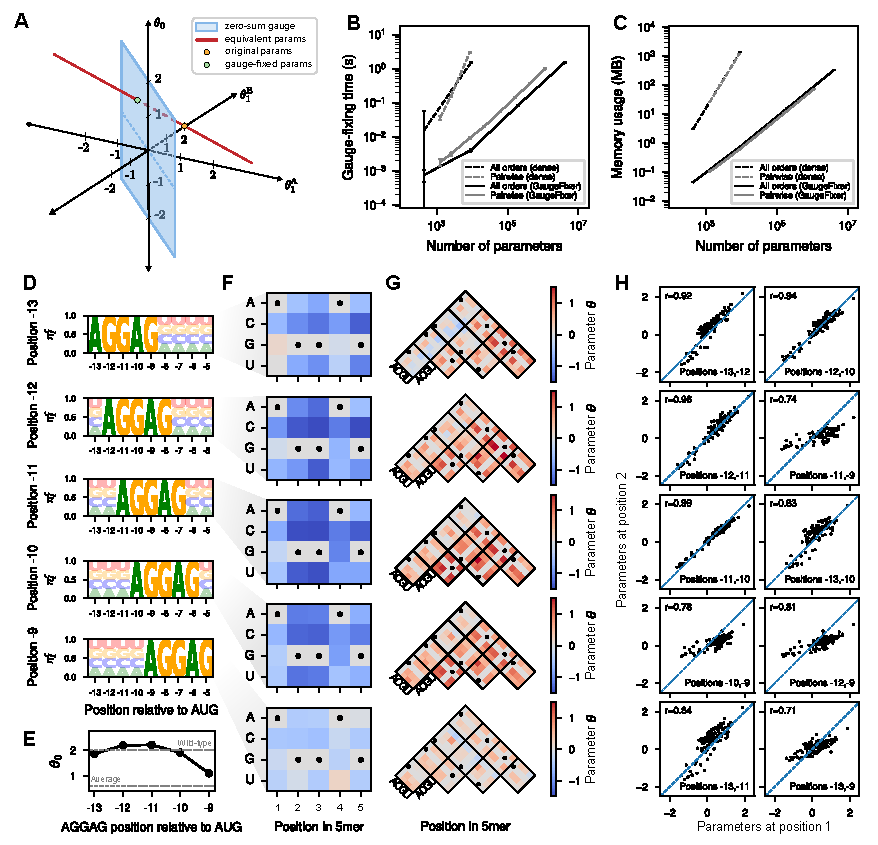
\includegraphics[width=\linewidth]{figures/Figure.png}
    \caption{GaugeFixer: a software package for fixing the gauge in sequence-function models with applications to the Shine-Dalgarno (SD) fitness landscape. 
    (A) Representation of the parameter subspaces for a sequence-function model with one site and two alleles. The red line represents the parameter subspace able to represent the phenotypes [-0.5, 1]. The plan represents the subspace of parameters in the zero-sum gauge. The two subspaces intersect at a unique point, where the model parameters are expressed in the zero-sum gauge.
    (B,C) Performance of GaugeFixer for fixing the gauge in all orders and pairwise interaction models in protein spaces with increasing number of parameters in terms of running time (B) and memory requirements (C), compared to a naive approach using dense projection matrices.
    (D) Sequence logos representing the site-independent probability distributions that represent the different peaks of the SD sequence with the AGGAG motif at different positions relative to the start codon. 
    (E,F,G) Representation of the gauge-fixed constant (E), additive (E) and pairwise (F) parameters, respectively, under the hierarchical gauge associated to each probability distribution associated to the AGGAG motif at different positions relative to the start codon AUG. Horizontal dashed lines in (E) represent the average phenotype across all possible sequences and the phenotype of the wild-type sequence AAGGAGGUG in the dmsC 5'UTR.
    (H) Scatterplots comparing the values of the gauge-fixed parameters of the local pairwise interaction model around each of the fitness peaks defined by the probability distributions in (D).}
    \label{fig:sd}
\end{figure*}

\section{Results}

\subsection{An efficient algorithm for fixing the gauge in all-order models}
% All order model with Kronecker factorization
Here, we present a new algorithm for projecting the parameters of any hierarhical linear model into a specific gauge with $O(M)$ memory and computational cost. To do so, we leverage the specific mathematical form of $P$, defined as tensor products of $L$ distinct subspaces of dimension $\alpha + 1$, one subspace for each position $l$. Consequently, the gauge-fixing projection matrix can be written as a Kronecker product of $L$ matrices:
\begin{align}
    P &= P_1 \otimes P_2 \otimes \cdots \otimes P_L, \label{eq:P_all_factorization}
\end{align}
where $P_k$ is a $(\alpha + 1) \times (\alpha + 1)$ position-specific projection matrix for any $k\in S$ as defined in \citet{Posfai2025aa}. Importantly, the product $P \vec{\theta}$ can be computed recursively using only one $P_k$ at a time~\citep{MartiGomez2025aa} (See Algorithm~\ref{alg:fix_gauge_all_orders}). We first reshape $\vec{\theta}$ to be an $L$-dimensional tensor having size $(\alpha+1)$ along each dimension. The expression in Eq. \ref{eq:theta_all_fixed} then becomes
\begin{align}
[\vec{\theta}_{\myfixed}]_{i_1 \cdots i_L} &= \sum_{j_1 \cdots j_L} [P_1]_{i_1 j_1} \cdots [P_L]_{i_L j_L} [\vec{\theta}]_{j_1 \cdots j_L} \label{eq:theta_fixed_kron}
\end{align}
where each $i$ and $j$ index $0, 1, \ldots, \alpha$. This can be computed by first defining $\vec{\theta}^{(0)} = \vec{\theta}$, then for $k=1,2,\cdots,L$ recursively computing
\begin{align}
\vec{\theta}^{(k)}_{i_1 \cdots i_L} = \sum_{j_k} [P_k]_{i_k j_k} [\vec{\theta}^{(k-1)}]_{i_1 \cdots i_{k-1} j_k i_{k+1} \cdots i_L}, \label{eq:P_i_prod}
\end{align}
where $\vec{\theta}^{(L)}$ corresponds to the gauge-fixed parameter vector $\vec{\theta}_\myfixed$.

\begin{algorithm}
    \caption{Fixing the gauge of all-order models}\label{alg:fix_gauge_all_orders}
    \begin{algorithmic}[1]
        \Require $\lambda,\pi,\vec{\theta}$
        \State $\vec{\theta}^{(k-1)} \gets \operatorname{reshape}(\vec{\theta})$
        \For{$k=1$ in $1$}
            \State $P_k \gets \operatorname{ProjectionMatrix}(\lambda, \pi_k)$ \Comment{\citet{Posfai2025aa}}
            \State $\vec{\theta}^{(k)} \gets \operatorname{tensordot}(P_k, \vec{\theta}^{(k-1)}, k)$ \Comment{Equation~\ref{eq:P_i_prod}}
            \State $\vec{\theta}^{(k-1)} \gets \vec{\theta}^{(k)}$
        \EndFor
        \State $\vec{\theta}_\myfixed \gets \operatorname{reshape}(\vec{\theta}^{(k)})$
    \end{algorithmic}
    \Return $\vec{\theta}_\myfixed$
\end{algorithm}

Note that equation~\ref{eq:P_i_prod} can be computed in practice as a tensor dot product of the $P_k$ matrix with the tensor $\vec{\theta}^{(k-1)}$. Thus, computation has complexity $O(L(\alpha+1) M)$, as opposed to $O(M^2)$ for the naive approach and memory requirements scale only linearly with the number of parameters $M$.

\subsection{Fixing the gauge in hierarchical models}

In this section, we present an extended algorithm that allows projecting the parameters of an arbitrary hierarchical model into a specific hierarhical gauge defined by $\pi$. We note that any hierarchical model can be decomposed as the sum of $m$ all-order interaction models defined over each of the generating orbits $U'\in W$ defined by $\vec{\theta}_{U'}$:
\begin{equation}
    \theta_U^u = \sum_{U'\in W:U\subseteq U'} [\vec{\theta}_{U'}]_U^u. \label{eq:hierarchical_decomposition}
\end{equation}
While this decomposition is not unique i.e. there are more parameters in the $m$ all-order models than in the hierarchical model, if the $m$ all-order models are expressed in a given gauge, any linear combination of them will also be in that gauge. Thus, we can take an arbitrary decomposition of $\vec{\theta}$ into the $\vec{\theta}_{U'}$, fix the gauge of the $\vec{\theta}_{U'}$ parameters using the Kronecker structure of the projection matrix $P_{U'}$ for the all-order model defined on each orbit $U'$ and add them up to obtain $\vec{\theta}_\myfixed$ using equation~\ref{eq:hierarchical_decomposition}. In practice, we do this via the following Algorithm~\ref{alg:fix_gauge_hierarchical} to avoid storing all $\vec{\theta}_{U'}$ simultaneously. 

% Hierarchical models can be decomposed as sums of all-order interaction models restricted to various subsets of positions. This is the strategy that GaugeFixer uses to handle hiderarhical models. [NEED TEXT DESCRIBING WHAT ORBITS ARE, AND WHAT GENERATING ORBITS ARE] With the generating set of orbits in hand, we can decompose the the parameter vector $\vec{\theta}_\myhier$ of the hierarchical model as a sum of $H$ all-order interaction parameter vectors restricted to the orbits $\tau_1, \cdots, \tau_H$: 
% \begin{equation}
%     \vec{\theta}_\myhier = \sum_{h = 1}^H \vec{\theta}_{\myall|\tau_h}. \label{eq:hierarchical_dot_decomposition}
% \end{equation}
% Gauge-fixing is then accomplished using the Kronecker factorization trick from Appendix \ref{appendix:all_order_model}:
% \begin{equation}
%     \vec{\theta}_\myfixed = \sum_{\sigma \in \mathcal{L}} P_{\myall|\sigma} \vec{\theta}_\sigma, \label{eq:theta_hierarchical_fixed}
% \end{equation}
% where each $P_{\myall|\sigma}$ is given by Eq.\ \ref{eq:P_all_factorization} restricted to the positions in $\sigma$. 

% In this section we use basic results from the theory of posets.\cite{Stanley2011aa} 

% Let $S$ denote the set of orbits (i.e., subsets of $\mathcal{L} = \set{1,2,\ldots,L}$) of a hierarchical model. Our first goal is to identify a minimal set of orbits $S_\mygen$ that is able to generate all orbits in $S$. In other words, $S_\mygen$ is the minimal set of orbits whose suboribts cover all orbits in $S$.  Because $\mathcal{L}$ is finite, it is readily proven that $S_\mygen$ exists, is unique, and comprises the antichain of maximal orbits in $S$. In many common cases $S_\mygen$ can be identified by inspection. Indeed, for any $K$-order or $K$-adjacent models, $S_\mygen$ is given  by the set of $K$-order orbits $S$. 

% For more complex models, $S_\mygen$ can be built iteratively. First we take $\tau_1$ to be a maximal-length orbit in $S$ and define $S_1 = S \setminus \mysubsets(\tau_1)$. Next we take $\tau_2$ to be a maximal-length orbit in $S_1$, define $S_2 = S_1 \setminus \mysubsets(\tau_2)$. Iterating until we encounter $S_H = \emptyset$ thus yields the generating set of orbits $S_\mygen = \set{\tau_1, \tau_2, \cdots, \tau_H}$.

%  Now, there is no unique way to decompose $\vec{\theta}_\myhier$. Moreover, we do not want to store all store all $\vec{\theta}_{\myall|\tau_h}$ as $H$ may be very large. 
%First, set $\vec{\theta}_\mysource = \vec{\theta}_\myhier$ and $\vec{\theta}_\mysink = \vec{0}$. Then for each $h = 1, \ldots, H$ do the following: $\vec{\theta}_h \leftarrow \vec{\theta}_{\mysource|T_h}$, $\vec{\theta}_\mysource \leftarrow \vec{\theta}_\mysource - \vec{\theta}_h$, $\vec{\theta}_{\myfixed,h} \rightarrow P_{\tau_h} \vec{\theta}_h$, $\vec{\theta}_{\mysink} \leftarrow \vec{\theta}_{\mysink}  + \vec{\theta}_{\myfixed,h}$.

\begin{algorithm}
    \caption{Fixing the gauge of hierarchical models}\label{alg:fix_gauge_hierarchical}
    \begin{algorithmic}[1]
        \Require $\pi,\vec{\theta},W$
        \State $\vec{\theta}_{\mysource} \gets \vec{\theta}$
        \State $\vec{\theta}_{\myfixed} \gets \vec{0}$
        \For{$U'$ in $W$}
            \State $\vec{\theta}_{U'} \gets \vec{\theta}_\mysource[U']$
            \State $[\vec{\theta}_{U'}]_\myfixed \gets \operatorname{FixAllOrder}(\infty, \pi[U'], \vec{\theta}_{U'}$) \Comment{Algorithm~\ref{alg:fix_gauge_all_orders}}
            \State $\vec{\theta}_\myfixed[U'] \gets \vec{\theta}_\myfixed[U'] + [\vec{\theta}_{U'}]_\myfixed$
            \State $\vec{\theta}_{\mysource}[U'] \gets \vec{0}$
        \EndFor
    \end{algorithmic}
    \Return $\vec{\theta}_{\myfixed}$
\end{algorithm}

\subsection{GaugeFixer: a software library for fixing the gauge in sequence-function models}
% High level explanation of the library
We have implemented these computationally efficient algorithms in a lightweight Python library called GaugeFixer. GaugeFixer provides a simple object-oriented interface, where users can define different classes of hierarchical models i.e. all-order, $K$-order, and $K$-adjancent interaction models, and project any set of previously inferred parameters into any user-defined gauge $\lambda ,\pi$ gauge for interpretation of their values.

To evaluate the performance of GaugeFixer's implementation, we computed the running time and memory requirements for fixing the gauge in different types of hierarhical models with increasing number of randomly initialized parameters (Figure~\ref{fig:sd}B and C). GaugeFixer shows over an order of magnitude increase in performance over the naive approach using a dense projection matrix and much better scaling with the number of parameters. 

\subsection{Analysis of the fitness landscape of the Shine-Dalgarno sequence}

To demonstrate the utility of GaugeFixer, we analyze the fitness landscape of the Shine-Dalgarno (SD) sequence, a 5' UTR motif that is critical for translation initiation in prokaryotes~\citep{Shine1975}. 
Using high-throughput fluorescence measurements of nearly every 9-mer~\citep{Kuo2020}, we previously inferred an all-order sequence-function model using variance component regression~\citep{Zhou2022} and showed that the landscape contains multiple peaks corresponding to recognition of the canonical motif at different distances from the start codon~\citep{MartiGomez2025aa}. Here, we use GaugeFixer to probe the local structure of each peak in more detail.

In order to define regions of sequence space corresponding to the different fitness peaks, we define a series of site-independent probability distributions $\pi$ with the AGGAG motif at different positions relative to the start codon. Thus, for a given position $p$, we set $\pi_{p}^{A}=1$, $\pi_{p+1}^{G}=1$, $\pi_{p+2}^{G}=1$, $\pi_{p+3}^{A}=1$, $\pi_{p+4}^{G}=1$, with all other sites drawn uniformly ($\pi_{l}^{c}=0.25$ for $l\notin [p, p+4]$, Figure~\ref{fig:sd}A). For each distribution, we fix the gauge using the hierarchical gauge ($\lambda=\infty$) to concentrate as much explanatory variance as possible into lower-order terms, and then interpret the resulting parameters. 

The zeroth-order parameter $\theta_0$ represents the mean phenotype under each distribution (i.e., the average fluorescence intensity of sequences with the AGGAG motif at the specified position). We find that $\theta_0$ is largest when the motif is at positions -12 and -11, consistent with an optimal SD positioning for translation initiation (Figure~\ref{fig:sd}E). In contrast, $\theta_0$ is much closer to the average intensity across all possible sequences for AGGAG motifs located at position -9, suggesting much weaker activation when binding at this position.
The parameters $\theta_{l}^c$ associated with the alleles at each position $l$ represent the average effect of fixing a allele $c$ when sequences are drawn from each probability distribution $\pi$. Our gauge-fixed $\theta_{l}^c$ show that the average allelic effects within the AGGAG motif are very similar across the different positions (Figure~\ref{fig:sd}F). These allelic effects are slightly different at position -13, where G is preferred at the first position of the 5-mer on average, and at position -9, where U is preferred over A at the fourth position. These differences could be driven by the presence of fixed alleles at positions -14 and -4 adjacent to the randomized motif, whereas the alleles at sites flanking the AGGAG motif at positions -12 to -10 are sampled uniformly.
Similarly, the parameters $\theta_{l_1 l_2}^{c_1 c_2}$ associated with pairs of alleles reflect the average deviation from the additive model when pairs of alleles are fixed in sequences drawn from the corresponding probability distributions. These parameters also show consistent patterns of interaction across the different positions and alleles (Figure~\ref{fig:sd}G), further supporting the similarity requirements around each of the peaks. These $\theta_{l_1 l_2}^{c_1 c_2}$ take mostly positive values, suggesting that combinations of mutations tend to have higher function than expected by their average single point mutational effects. 

These constant, additive and pairwise interaction terms define a local pairwise interaction model for the sequence requirements at each binding register. Figure~\ref{fig:sd}H quantitatively compares the parameters of these models across every pair of binding positions. These results show that the local sequence-function models around each peak are more similar between neighboring positions, and differ as they become far appart in the primary sequence, suggesting that binding preferences change smoothly as a function of the distance to the start codon.
While the parameters of the local model at position -9 are in general of smaller magnitude, they remain substantially correlated with the model parameters for the other positions (Figure~\ref{fig:sd}H). 
%Together with the lower average function of AGGAG motifs at position -9 (Figure~\ref{fig:sd}E) and the predominantly positive pairwise parameters (Figure~\ref{fig:sd}G), it suggests a global scaling of the effects of mutations with the background phenotype i.e. global epistasis. % not sure we need to get into this 

In summary, GaugeFixer allowed us to explore and compare the structure and sequence determinants of the different peaks in the Shine-Dalgarno fitness landscape, uncovering similarities and differences in the recognition modes at different positions relative to the start codon.


% \begin{table*}[t]
% \centering
% \small
% \begin{tabular}{|c|c|c|c|c|c|}
% \hline
% \multicolumn{1}{|c|}{} & \multicolumn{1}{c|}{} & \multicolumn{2}{c|}{\textbf{memory usage}} & \multicolumn{2}{c|}{\textbf{multiplication operations}} \\
% \cline{3-6}
% \multicolumn{1}{|c|}{\textbf{model type}} & \textbf{num. parameters ($M$)} & \textbf{standard} & \textbf{Kronecker} & \textbf{standard} & \textbf{Kronecker} \\
% \hline
% additive & 
%     $1 + \alpha L$ &
%     $M^2$ & 
%     $L (\alpha+1)^2$ & 
%     $M^2$ &
%     $(\alpha+1) M$ \\
% neighbor & 
%     $1 + \alpha L + \alpha^2 (L-1)$ &
%     $M^2$ &
%     $L(\alpha+1)^2$ &
%     $M^2$ &
%     $2 (L-1) (\alpha+1) M$ \\
% pairwise & 
%     $1 + \alpha L + {L \choose 2}\alpha^2$ &  
%     $M^2$ &
%     $L(\alpha+1)^2$ & 
%     $M^2$ & 
%     $2 {L \choose 2} (\alpha+1) M$ \\
% all-order & 
%     $(\alpha+1)^L$ &  
%     $M^2$ & 
%     $L(\alpha+1)^2$ & 
%     $M^2$ & 
%     $L (\alpha+1) M$ \\
% $K$-order & 
%     $\sum_{k=0}^K {L \choose k}\alpha^k$ & 
%     $M^2$ & 
%     $L(\alpha+1)^2$ & 
%     $M^2$ &
%     $K {L \choose K} (\alpha+1) M$ \\
% $K$-adjacent & 
%     $ (\alpha + 1)^K + (L-K)\sum_{k=1}^K {K-1 \choose k-1}\alpha^k $ & 
%     $M^2$ & 
%     $L(\alpha+1)^2$ &
%     $M^2$ & 
%     $K (L-K+1) (\alpha+1) M$ \\
% \hline
% \end{tabular}
% \caption{Memory and computational requirements for gauge-fixing different model types using naive versus fast (Kronecker factorization) approaches. Here $M$ is the total number of model parameters, $L$ is sequence length, $\alpha$ is alphabet size, and $K$ is interaction order.}
% \label{tab:complexity}
% \end{table*}

% \begin{figure*}[t]
%     \centering
%     \includegraphics[width=6.5in]{fig1_resources}
%     \caption{Resource requirements for gauge-fixing different model types. (a) Memory usage and (b) number of multiply operations required by naive versus fast (Kronecker factorization) approaches. Here $M$ is the total number of model parameters, $L$ is sequence length, $\alpha$ is alphabet size, and $K$ is interaction order.}
%     \label{fig:resources}
% \end{figure*}

\section{Discussion}
Here we introduced GaugeFixer, a lightweight Python library that implements a computationally efficient algorithm for removing unconstrained degrees of freedom (``fix the gauge'') from the parameters of a wide range of linear sequence-to-function models. By exploiting the Kronecker factorization of projection operators and the structure of hierarchical models, our new algorithm reduces the time and memory complexity of gauge fixing from $O(M^2)$ to $O(M)$, making it practical for models with millions of parameters. 

It is important to emphasize that gauge fixing is completely independent from parameter inference. Although particular regularization schemes or prior distributions can implicitly pick out a gauge during model fitting \citep{Posfai2025aa,Petti2025aa}, fixing the gauge is a separate post-processing step applied to an already-specified model. GaugeFixer makes this distinction explicit by providing utilities to convert any precomputed parameter vector into a series of different gauges for interpretation.

Gauge fixing can in principled be applied for interpretation of nonlinear and nonparametric models, such as neural networks or Gaussian process models, by representing them as all-order linear models. In this work we used GaugeFixer to extract gauge-fixed parameters from a Shine-Dalgarno sequence-function model inferred using Gaussian process regression \citep{Zhou2022,MartiGomez2025aa} allowing us to zoom in into the local sequence requirements in different regions of sequence space. This feasible when sequences are short enough to enumerate the parameters associated to features of every possible order. However, recent theoretical results \citep{Petti2025aa} further show that gauge-fixed parameters can be computed for a broad class of Gaussian process models with site-wise product kernels defined over sequences of arbitrary length, opening a practical route to interpret these powerful nonparametric models.

In summary, GaugeFixer provides the first softare library for fixing the gauge of linear models, filling an important gap in the set of computational tools for interpreting models of sequence-function relationships.

%%%%%%%%%%%%%%

% \begin{appendices}

% \end{appendices}

\section{Competing interests}
The authors declare no competing interests. 

\section{Author contributions statement}
C.M-G. and J.B.K concieved the project, wrote the package, and performed the research. C.M-G., D.M.M, and J.B.K. wrote the manuscript. J.B.K supervised the research. 

\section{Acknowledgments}
This work was supported in part by: NIH grants R01HG011787 (J.B.K, D.M.M.), R35GM133777 (J.B.K.), and R35GM133613 (D.M.M., C. M-G.). Computational equiptment was supported by NIH grant S10OD028632.

\bibliography{reference}
\end{document}
